\section{Quadcopter Design}
This section describes the concept designs and builds of the quadcopters and parts. 

\subsection{Considerations}
When constructing a quadcopter, special considerations must be made concerning weight, weight distribution and vibrations. There are also many other important design factors, but the mentioned above are the most important for this project.  

\subsection{Components and Manufacture}
In this project a combination of commercially available components and self made parts will be used. Motors, servos, propellers and electronics will be bought.
\\\\
A laser-cutter and 3D-printer is at the teams disposal, which ensures rapid prototyping. At campus, the team has access to a small manual milling machine, lathe and drilling machine. The composites laboratory at campus may also be utilized if needed.

\subsection{Fixed Pitch Quadcopter Design Concepts}
At the beginning of the project, the team had intentions of making two similar quadcopters with less than 11 inch propellers. One fixed pitch quadcopter and one variable pitch quadcopter. The quadcopters should have motors with interchangeable fixed and variable pitch mechanisms. The reason is to achieve maximum similarity to get the best foundation for comparison. 
\\\\
An order was placed for motors of the type AEO C20 that could handle both fixed and variable pitch with minor modifications. The first motors and mechanisms that were obtained, were not usable because of bad quality. Due to limited time and no working fixed pitch quadcopter to test the code and control system on, the team used the resources available and borrowed a set of DJI E600 motors with 12 inch propellers.
\\\\
This was the fastest and most economical way of creating a fixed pitch quadcopter until new variable pitch mechanisms and motors were acquired.
\\\\
For the DJI E600 motors, two quadcopter concepts were made. 
\begin{figure}[h]
        \centering
         \begin{minipage}[b]{0.45\textwidth}
            \includegraphics[width = 1\textwidth]{VAPIQ-PICTURES/FixedPitchConceptCarbon}
              \caption{Fixed Pitch Carbon and 3D-print Model}
            \label{fig:CarbonFPQ}
        \end{minipage}
        \hfill
        \begin{minipage}[b]{0.45\textwidth}
            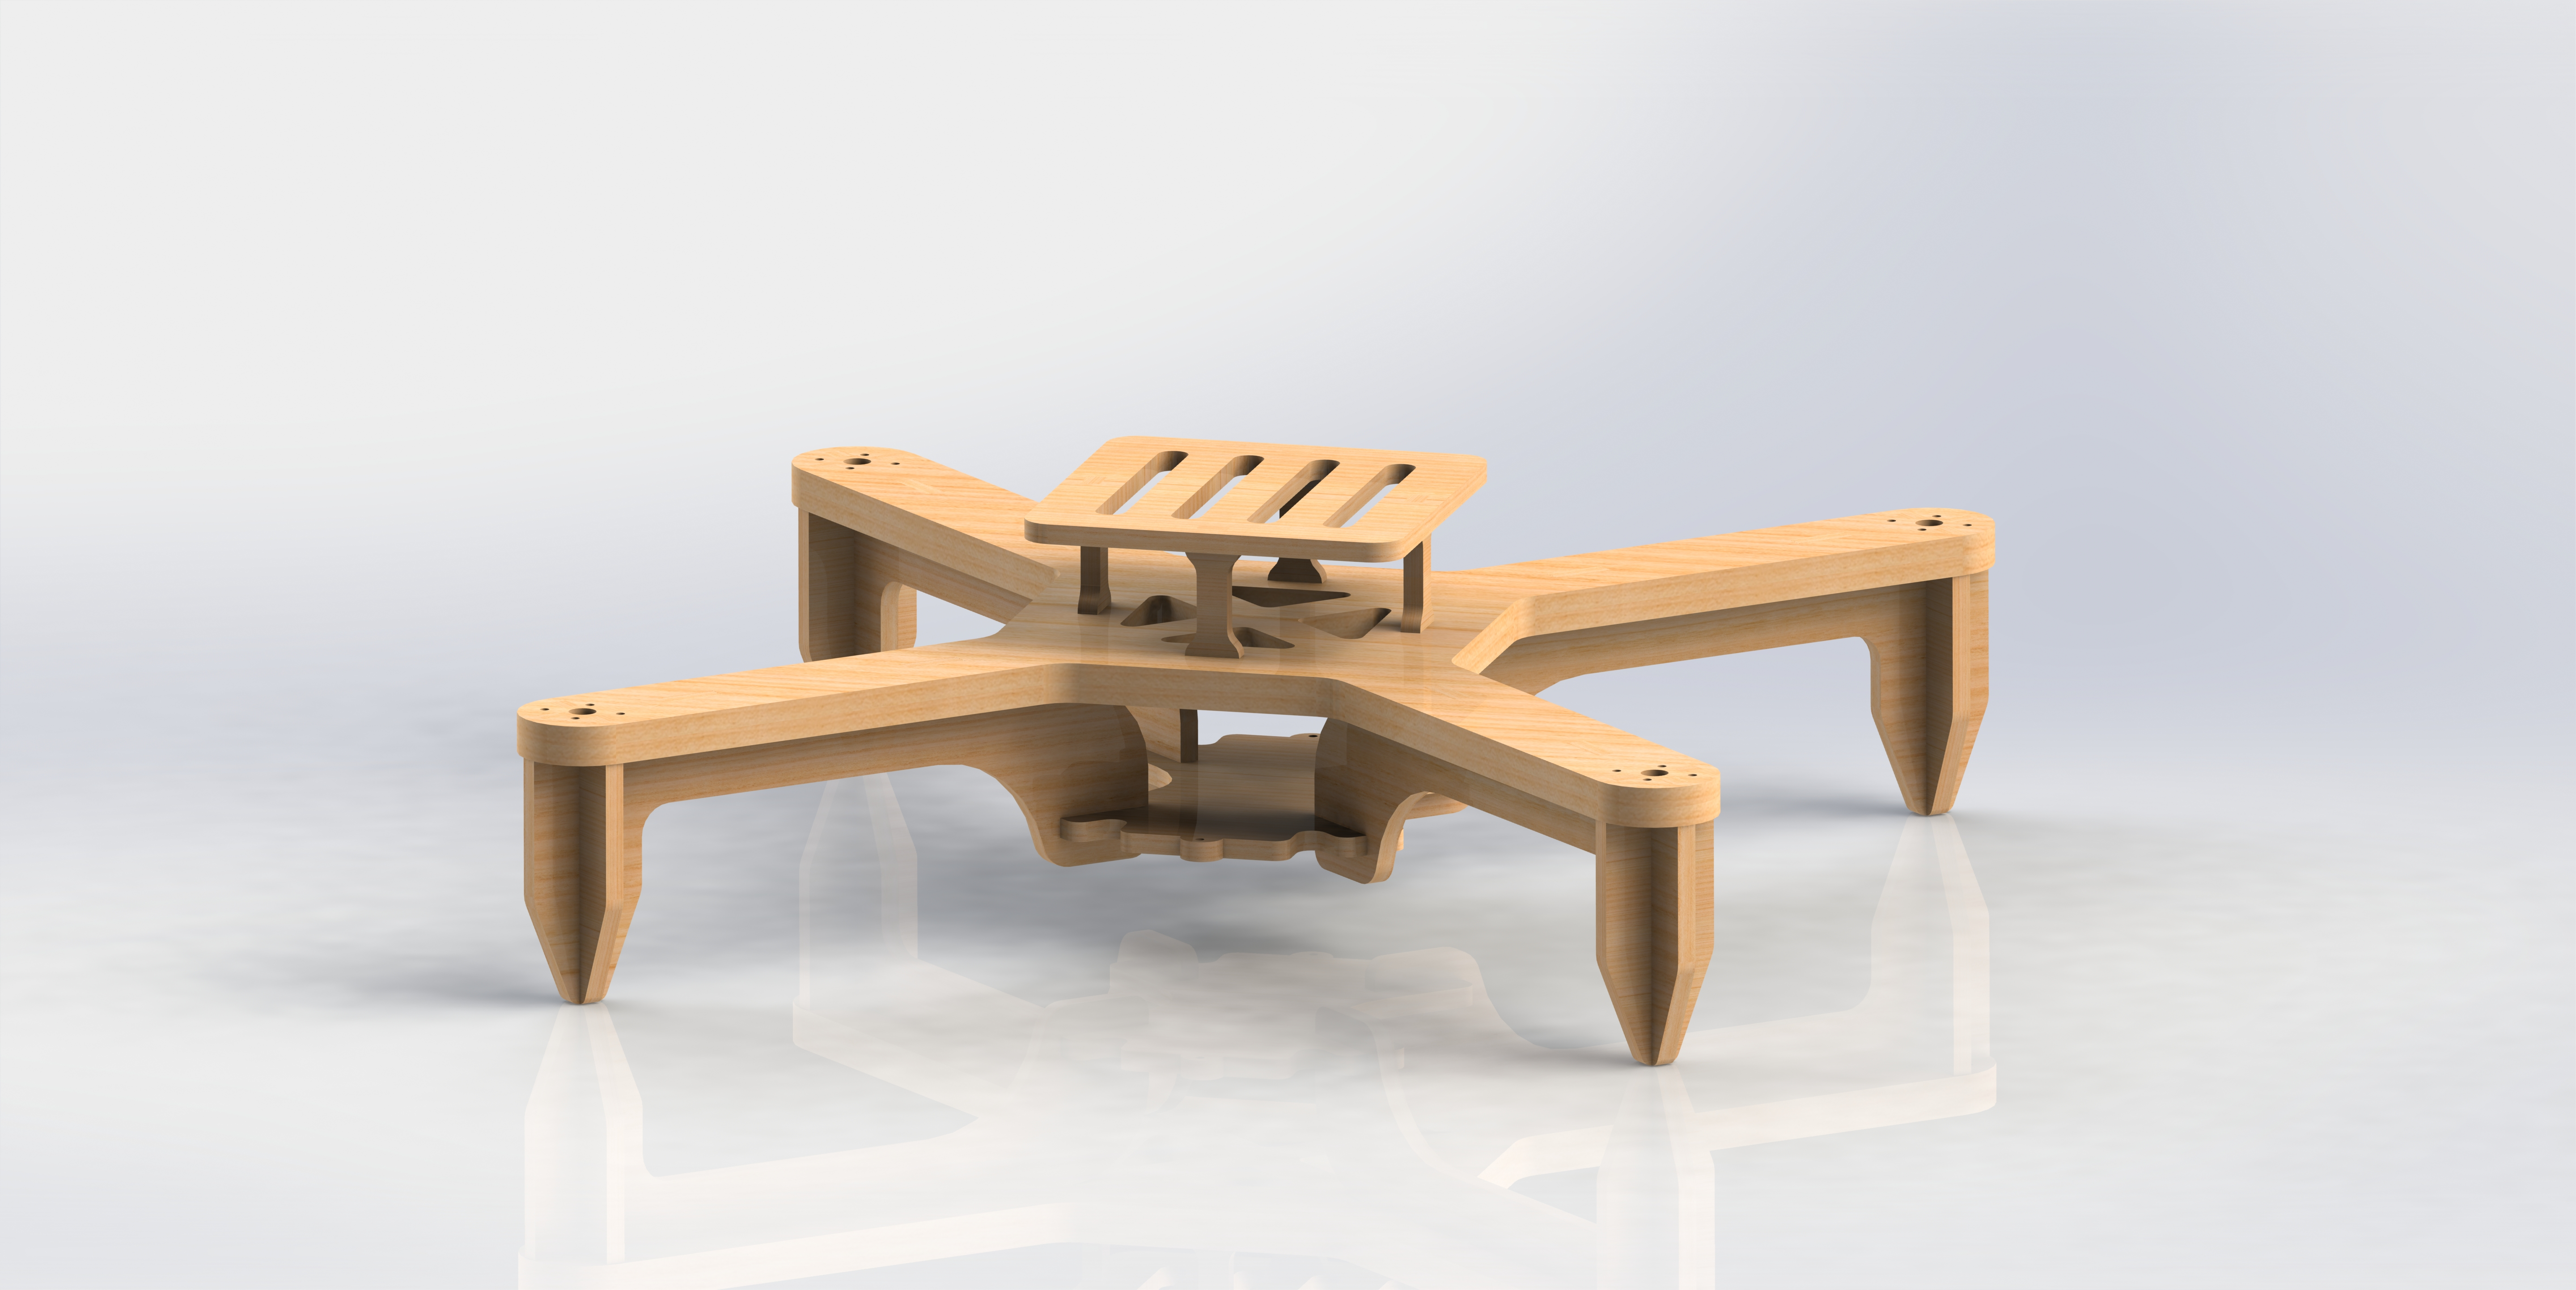
\includegraphics[width = \textwidth]{VAPIQ-PICTURES/FixedPitchso2}
            \caption{Fixed Pitch Plywood Model}
            \label{fig:FPQply}
        \end{minipage}
\end{figure}

\noindent
The concept chosen for the fixed pitch quadcopter was the Plywood Model, see Fig. \ref{fig:FPQply}. This design was the fastest to manufacture and the most economical to build. The entire quadcopter frame, support legs and battery holder is made completely with 6,5 mm plywood plates, and can be cut in a single session in a laser-cutter. 
\\\\
The build consists of two 6,5 mm main plates glued together with slots for mounting the support legs and top-plate supports. The support legs consists of two parts. One long part, acting as a structural stiffener and as a mount for the battery plate. The second part of the leg is short and perpendicular to the long part for lateral support.
\\\\
For the carbon fixed pitch quadcopter, the frame is made up of two custom cut 2,0 mm carbon fiber plates and 20 mm diameter carbon fiber tube arms. To secure the tube arms, a double set of 3D-printed tube clamps are placed between the custom plates. At the end of the tube arms, there are 3D-printed brackets for the support legs which also acts as a brackets for the motor mount plates. The support legs and motor mount plates, are either 3D-printed or laser-cut, but could also be cut from carbon or glass fiber plates. The battery is placed with a battery strap, through custom slots on the underside of the quadcopter.
\\\\
Since the main objective of this bachelors thesis is not to build a fixed pitch quadcopter, the plywood model was chosen to free time and resources for the variable pitch quadcopter.

\subsection{Fixed Pitch Quadcopter Build}

The plywood quadcopter was manufactured using an Epilog 65W laser-cutter at KIC. After cutting, the quadcopter was glued, assembled and electronics were installed (Fig. \ref{fig:Assey}). The E600 motors have a maximum thrust of 1600g/axis, giving the quadcopter a total capacity of 6,4 kg thrust. The assembly has a total weight of 1856g, giving the quadcopter a power to weight ratio of approximately 3,4.

\begin{figure}[h]
        \centering
         \begin{minipage}[b]{0.3\textwidth}
            \includegraphics[width = 1\textwidth]{VAPIQ-PICTURES/LaserCut}
              \caption{Cutting quadcopter with Epilog 65W laser}
            \label{fig:CarbonFPQ}
        \end{minipage}
        \hfill
        \begin{minipage}[b]{0.65\textwidth}
            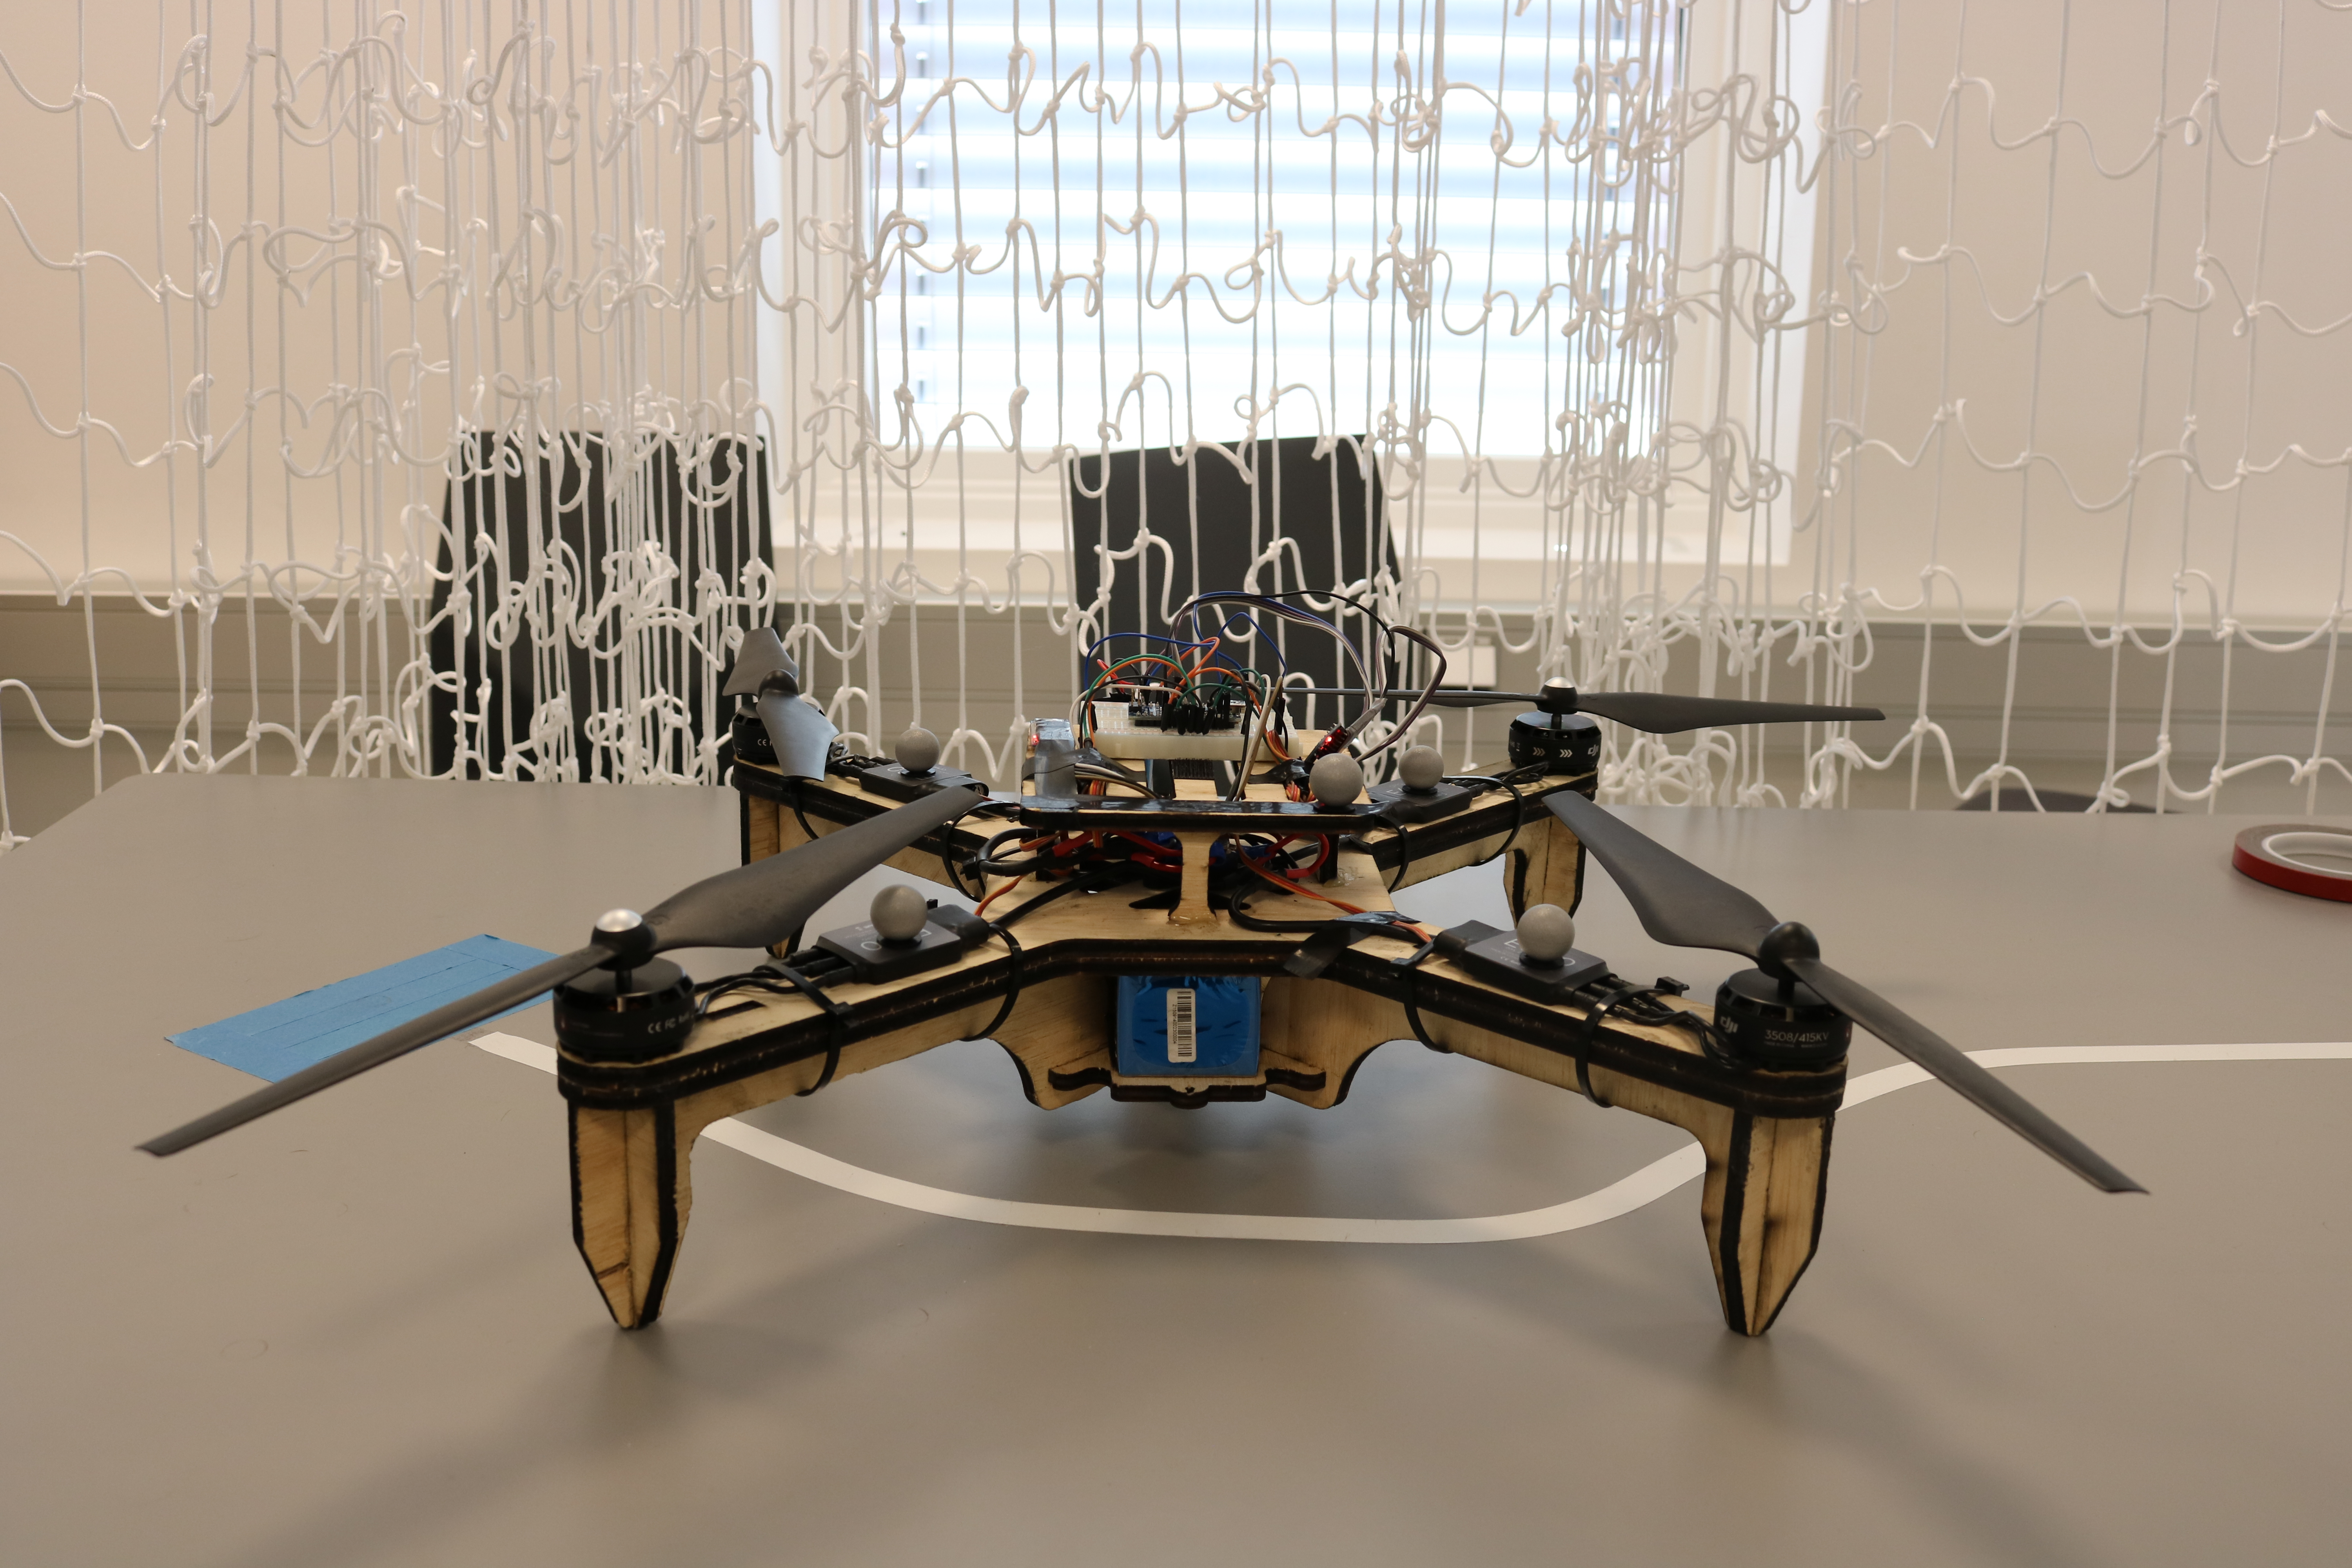
\includegraphics[width = \textwidth]{VAPIQ-PICTURES/AssembledFPQ}
            \caption{Fully assembled fixed pitch quadcopter}
            \label{fig:Assey}
        \end{minipage}
\end{figure}


%%%%%%%%%%
%- Hardware list
%- Mass budget, ish for fixed
%- Power to wheight? ish chack
%%%%%%%%%%
\newpage
\subsection{Variable Pitch Concept 1}

The first concept for the variable pitch quadcopter, was to rebuild a 3DR Arducopter Frame, see Fig. \ref{fig:Arducopter}. The concept consists of adding helicopter tail pitch mechanisms with mounted motors underneath. Modifying the tail mechanisms, changing the square arms with carbon fiber tubes, adding tube clamps, leg brackets, servo holders and linkage rods (Fig. \ref{fig:Arducopter}). 
\begin{figure}[h]
        \centering
         \begin{minipage}[b]{0,35\textwidth}
            \includegraphics[width =\textwidth, angle =0]{VAPIQ-PICTURES/3DRArducopterCframeKit}
              \caption{3DR Arducopter C Frame Kit}
           \label{fig:Arducopter}
        \end{minipage}
        \hfill
        \begin{minipage}[b]{0.35\textwidth}
            \includegraphics[width = \textwidth]{VAPIQ-PICTURES/ModForVPQ}
            \caption{Parts For Quadcopter Rebuild}
           \label{fig:PartsForArdu}
        \end{minipage}
\end{figure}

\noindent
The tube clamps holds the tubes in place and are mounted between the main plates of the frame. Underneath the tube clamp, the leg bracket is mounted. On the tube arms, a servo holder keeps the servo in position, and from the servo, a linkage rod transfers force to adjust the pitch of the propellers.
\\\\
The legs were moved towards the center of the quadcopter to compensate for the added weight from the motors and mechanisms. The addition of the variable pitch mechanisms, servos and motors affects the weight  distribution of the quadcopter, thus increasing the rotational inertia. The fasteners used in this build are M3 screws and bolts, and all the parts in (Fig. \ref{fig:PartsForArdu}) excluding the carbon tubes are 3D-printed. 
\newpage
\subsection{Helicopter Tail Pitch Mechanism}

Four variable pitch mechanisms were made using RC helicopter tails of the type HK500GT, steel rods and 880KV motors.

\begin{figure}[h]
        \centering
         \begin{minipage}[b]{0,6\textwidth}
            \includegraphics[width =\textwidth, angle =180]{VAPIQ-PICTURES/VPQParts}
              \caption{3DR 880KV motor, 4mm steel rod, hk500gt tail assembly}
            \label{fig:nlknl}
        \end{minipage}
        \hfill
        \begin{minipage}[b]{0.35\textwidth}
            \includegraphics[width = \textwidth]{VAPIQ-PICTURES/VPQassemblies}
            \caption{Assemblies}
            \label{fig:}
        \end{minipage}
\end{figure}

\noindent The mechanisms were built using 4 mm diameter stainless steel rods which runs through the motor and mechanism. The rods are precision cut from a 3 m specimen into 4 pieces of 92,5 mm in length. 

\begin{figure}[H]
        \centering
         \begin{minipage}[b]{0,35\textwidth}
            \includegraphics[width =\textwidth, angle =270]{VAPIQ-PICTURES/Drilling}
              \caption{Drilling}
            %\label{fig:nlknl}
        \end{minipage}
        \hfill
        \begin{minipage}[b]{0.35\textwidth}
            \includegraphics[width = \textwidth, angle= 270]{VAPIQ-PICTURES/latheWork}
            \caption{Lathe Work}
            %\label{fig:}
        \end{minipage}
\end{figure}
\noindent
The motor is mounted through two custom drilled holes with M3 screws and bolts. Using a lathe machine, grooves were made in the shafts to hold the C-clips which ensures that the shaft does not slide. To fit the shafts through the motor, a press machine was used.

\subsection{Concept 1, Conclusion}

Calculation of the thrust forces produced by the motor-propeller combination was difficult to estimate theoretically. Therefore, thrust had to be measured empirically by using a test rig. The maximum thrust produced in the test rig was approximately 700g on 4 cell battery voltage, giving a max thrust of 2,4 kg. The problem was that the motor drew 18,6 A of current and quickly became overheated. The mass estimate of the quadcopter assembly was 1,8kg, leaving only 600g of spare thrust on maximum power and a power to weight ratio of 1,3. These factors resulted in the concept being discarded.
\\\\
From the motors with the tail pitch mechanisms, there was built a one-axis test rig. This was done so experimentation on stabilization of variable pitch could continue until the variable pitch quadcopter was finished. 

\begin{figure}[H]
    \centering
         \includegraphics[width = 0.8\textwidth]{VAPIQ-PICTURES/VPQ_rainbow_Rig.jpg}
      \caption{One-Axis Variable Pitch Test Rig}
   % \label{fig:}
\end{figure} 


% Legge inn rainbow testing rig; for testing variable pitch stabilization.

\subsection{Variable Pitch Concept 2}

After receiving the AXI 2208/26 motors with variable pitch mechanisms, a new concept had to be made. The new motors can produce approximately 500g of thrust each, giving a total lift of 2 kg.
\\\\
The concept consists of designing a frame that can hold all components, but as light as possible to achieve the highest power to weight ratio. The frame will be made from hybrid carbon fiber sandwich material, where the soft core material is PVC foam and the outer stiff material is carbon fiber with 12k weave and (0,90) fiber orientation.
\\\\
Legs with servo holders, as well as component brackets will be 3D-printed.

\begin{figure}[H]
        \centering
                \begin{minipage}[b]{0.4\textwidth}
            \includegraphics[width = \textwidth, angle= 0]{VAPIQ-PICTURES/MakingVPQFrame.PNG}
            \caption{Making VPQ Frame}
            %\label{fig:}
                    \end{minipage}
                 \hfill
         \begin{minipage}[b]{0,35\textwidth}
            \includegraphics[width =\textwidth, angle =0]{VAPIQ-PICTURES/VacumInfusionVPQFrame.PNG}
              \caption{Vacum Infusion of VPQ frame}
            %\label{fig:nlknl}
        \end{minipage}

\end{figure} 
% abbreviation MDF- medium density fiber?
\noindent

The frame was manufactured using a laser cut model made from MDF(Medium Density Fiber). The MDF-model was used as a outline for cutting foam and the carbon fiber cloth. The build is hand traced and cut. After gluing the carbon fiber on each side of the foam, the construction was infused with epoxy resin under vacuum and left to cure for 48 hours. Five holes were drilled at the end of each quadcopter arm for mounting the motors. 

\begin{figure}[H]
        \centering
                \begin{minipage}[b]{0.3\textwidth}
            \includegraphics[width = \textwidth, angle= 0]{VAPIQ-PICTURES/ServoMountRender.jpg}
            \caption{Servo Mount}
            \label{fig:Bracket}
                    \end{minipage}
                 \hfill
         \begin{minipage}[b]{0.5\textwidth}
            \includegraphics[width = \textwidth, angle =0]{VAPIQ-PICTURES/vpqquad}
              \caption{Finished Variable Pitch Quadcopter}
            %\label{fig: Finished Shit}
        \end{minipage}
        \end{figure}


Servos are mounted directly beneath the motor in a 3D-printed bracket(Fig:\ref{fig:Bracket}) which also acts as legs for the quadcopter. In front of the bracket in figure:\ref{fig:Bracket} the servo linkage arm, this arm connects to a ball head screw on the servo horn and is attached to the variable pitch mechanism. On the top of the quadcopter a laser cut plywood piece is mounted on nylon standoffs to accommodate for all the electronics.


%stiffens/wheigt

\newpage

\subsection{Mechanical Challenges}


After the variable pitch quadcopter frame and components were mounted, the drilled holes were somewhat imprecise. This imprecision contributed to friction between the motor and frame, which in turn resulted in heating.\\
\\
The temperature of the motors must have exceeded the glass-liquid transition temperature of the polyvinyl chloride-foam in the core material of the frame (Approx.82 °C). The glass-liquid transition temperature is the temperature at which an amorphous material goes from a hard solid state to a more viscous or rubbery state where it is more easily susceptible to deformations. \\
\\
It is observed that the frame has deformations where the motors are mounted. This deformation has occurred because of the elevated temperatures and the high pressure zones under the motors. The high temperature in combination with pressure between the motor and frame has given permanent deformations and has caused the motors to come out of alignment.  \\
\\
To solve the alignment issue, four pieces of laser cut MDF brackets were mounted between the frame and motor. The plate has more surface area than the motor itself which helps distribute the pressure and align the motor, they also insulate the frame from the high temperatures developed by the motors.\\
\\
Additionally, all the holes were sanded down to eliminate the friction. \\
\\

\begin{figure}[H]
    \centering
         \includegraphics[width = 0.3\textwidth]{VAPIQ-PICTURES/MDFmotorPlate}
      \caption{MDF-Motor Mount}
   % \label{fig:}
\end{figure} 

Ideally, the frame should be remade with a more heat resistant core material or with pure carbon plates which are less susceptible to temperature related deformations. The frame should also be CNC (Computer Numerical Control) machined to ensure absolute precision. If there is time, a new frame will be constructed.\\
\\
Another challenge with the variable pitch quadcopter is the placement of the servos and the linkage between the servos and motors. \\
\\
The positioning and linkage must be as precise as possible to ensure the best possible power transfer to the pitch mechanism. If the position of the servos and linkage are not precise, it could result in the servo dragging the inner shaft out of position further increasing vibrations and wear in the system. Additionally, controlling the quadcopter will be more difficult if the servos are not giving the same mechanical output to the pitch mechanism when actuated.

%- Counter Measures

\newpage


